\section{Light-emitting diode (LED)}

%----------------------------------------------------------------------------------------
%	DEFINITION SUBESCTION
%----------------------------------------------------------------------------------------
\subsection{Definition}
A light-emitting diode (LED) is a two-lead semiconductor light source. It is a p–n junction diode, which emits light when activated.[4] When a suitable voltage is applied to the leads, electrons are able to recombine with electron holes within the device, releasing energy in the form of photons. This effect is called electroluminescence, and the color of the light (corresponding to the energy of the photon) is determined by the energy band gap of the semiconductor.\\


\centerline{
	\centering
	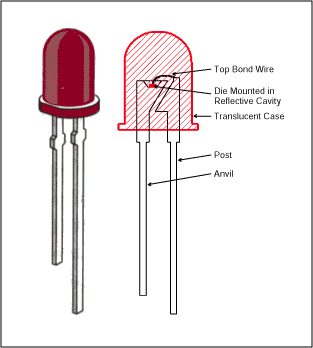
\includegraphics[width=0.8\textwidth]{overview/images/led.png}
}

%----------------------------------------------------------------------------------------
%	USAGE SUBESCTION
%----------------------------------------------------------------------------------------

\subsection{Usage}
Early LEDs were often used as indicator lamps for electronic devices, replacing small incandescent bulbs. They were soon packaged into numeric readouts in the form of seven-segment displays, and were commonly seen in digital clocks.

